\documentclass{handout}

% \SetInstructor{Lt Col James Phillips}
\SetCourseTitle{ECE231: Electrical Circuits and Systems I}
\SetSemester{Block III}
\SetHandoutTitle{Lecture 31: Energy and Power in the Phasor Domain}

%\SetDueDate{1 Jan 2016}
%\ShowAllBlanks

\showsoln \setsolncolor{red}

\begin{document}
\maketitle

\textbf{OBJECTIVES:}
\begin{enumerate}
\item .....
\end{enumerate}

\textbf{READING}
\begin{description}
\item [Required]:
Textbook, section 8.6, pages 431--436
\item [Optional]:
\end{description}

\section{Introduction \& Review}
Today we are going to look at power and energy in {\em RLC} circuits.  The analysis will all be done in the phasor domain.  Before we tackle new material, lets look back at our eariler lessons on power.

From early in the class (and from Physics) we should know that power is energy per time; expressed mathematically:
\begin{equation}
p(t) = \frac{\partial}{\partial t}w(t)
\label{eq: PE}
\end{equation}
where $p(t)$ is power as a function of time and $w(t)$ is energy as a function of time.

We also learned early in the class that power is the product of votage and current:
\begin{equation}
p(t) = v(t)i(t)
\label{eq: Power}
\end{equation}

Using Ohm's law we can write an expression for power in a resistor as:
\begin{equation}
p(t)=i^2(t)R
\label{eq: ResistorPower}
\end{equation}
or
\[
p(t)=\frac{v^2(t)}{R}
\]

For capacitors we recall (from lesson 20) that:
\begin{equation}
p(t) = \frac{\partial }{\partial t}\left[ \frac{1}{2}Cv^2(t) \right]
\label{eq: CapPower}
\end{equation}

For inductors we recall that:
\begin{equation}
p(t) = \frac{\partial }{\partial t}\left[ \frac{1}{2}Li^2(t) \right]
\label{eq: IndPower}
\end{equation}

This gives us a great starting point for our new material.

\section{Energy and Power in Resistors}
If we assume a current of $i(t)=I_A\cos(\omega t)$ through a resistor, the power consumed is:
\soln{0.75in}{
\[
p_R(t) = I_A^2R\cos^2(\omega t)
\]
}
given that $\cos^2\theta = \frac{1}{2}\left[ 1+\cos 2\theta \right]$ we can rewrite this as:
\soln{0.75in}{
\[
p_R(t) = \frac{I_A^2R}{2}\left[ 1+\cos(2\omega t)\right]
\]
}
which expands to:
\soln{0.75in}{
\[
p_R(t) = \frac{I_A^2R}{2}+\frac{I_A^2R}{2}\cos(2\omega t)
\]
}

So, for a sinusoidal current (or voltage), the power consumed in a resistor has 2 parts: An constant component and a sinusoidal component at twice the orginal frequency!

We can use equation \ref{eq: PE} to solve for the energy delivered to the resistor $w_R(t)$:
\[
w(t) = \int p(t) \partial t
\]
\soln{1in}{
\[
\int p_R(t) \partial t = \int \left[\frac{I_A^2R}{2}+\frac{I_A^2R}{2}\cos(2\omega t)  \right]\partial t
\]
which gives
\[
w_R(t) = \frac{I_A^2Rt}{2} + \frac{I_A^2R}{4\omega}\sin(2\omega t)
\]
}

Notice that $w_R(t)$ is montonic (increasing) and increases without bound.  Resistors always absorb energy and the longer current is applied, the more energy is absorbed!

\newpage
\clearpage
\pagebreak

\section{Energy and Power in a Capacitor}
For this quick derivation, let's start with equation \ref{eq: CapPower} and assume an AC voltage of the form $v(t) = V_A\cos(\omega t)$:
\soln{1in}{
\[
p_C(t) = \frac{\partial }{\partial t}\left[ \frac{1}{2}CV_A^2\cos^2(\omega t) \right]
\]
}

Using the same trig identity from above, we can rewrite this as:
\soln{1in}{
\[
p_C(t) = \frac{\partial }{\partial t}\left[ \frac{1}{4}CV_A^2\left[1+\cos(2\omega t)\right] \right]
\]
}

If we integrate both sides (from equation \ref{eq: PE}) we get the energy delivered to the capacitor:
\soln{1in}{
\[
w_C(t) = \frac{1}{4}CV_A^2\left[1+\cos(2\omega t)\right]
\]
}

If instead of integrating our expression for $p_C(t)$, we go ahead and do the time derivative, we get instantaneous power in the capacitor:
\soln{1in}{
\[
p_C(t) = -\frac{\omega CV_A^2}{2}\sin(2\omega t)
\]
}

\textbf{What have we learned from these equations?}
\soln{2in}{
\begin{enumerate}
\item The average power consumed/delivered by a capacitor is zero (more on this later)
\item The energy stored by a capacitor is a sinusoidal function.  When the function is increasing, the capacitor is absorbing power.  When the function is decreasing, the capacitor is delivering power to the circuit
\item The power and energy are $90^o$out of phase with one another ($\cos$ and $\sin$)
\end{enumerate}
}


\newpage
\clearpage
\pagebreak

\section{Energy and Power in an Inductor}
For this quick derivation, let's start with equation \ref{eq: IndPower} and assume an AC current of the form $i(t) = I_A\cos(\omega t)$:
\soln{1in}{
\[
p_L(t) = \frac{\partial }{\partial t}\left[ \frac{1}{2}LI_A^2\cos^2(\omega t) \right]
\]
}

Using the same trig identity from above, we can rewrite this as:
\soln{1in}{
\[
p_L(t) = \frac{\partial }{\partial t}\left[ \frac{1}{4}LI_A^2\left[1+\cos(2\omega t)\right] \right]
\]
}

If we integrate both sides (from equation \ref{eq: PE}) we get the energy delivered to the capacitor:
\soln{1in}{
\[
w_L(t) = \frac{1}{4}LI_A^2\left[1+\cos(2\omega t)\right]
\]
}

If instead of integrating our expression for $p_C(t)$, we go ahead and do the time derivative, we get instantaneous power in the capacitor:
\soln{1in}{
\[
p_L(t) = -\frac{\omega LI_A^2}{2}\sin(2\omega t)
\]
}

\textbf{What have we learned from these equations?}
\soln{2in}{
\begin{enumerate}
\item The average power consumed/delivered by an inductor is zero (more on this later)
\item The energy stored by a inductor is a sinusoidal function.  When the function is increasing, the inductor is absorbing power.  When the function is decreasing, the inductor is delivering power to the circuit
\item The power and energy are $90^o$out of phase with one another ($\cos$ and $\sin$)
\end{enumerate}
}

\newpage
\clearpage
\pagebreak

\section{Average Power}
As seen above, power is a time dependent variable; however, often we are only interested in average power.  To solve for average power (over a given interval) we use:
\soln{1in}{
\[
P_{AVE} = \frac{1}{T_0}\int_0^{T_0} p(t) \partial t
\]
}
where $T_0$ is the period.

\subsection{Resistor Average Power}
If we plug the resistor power equation and solve for average power we get:
\soln{2in}{
\[
P_{AVE-R} = \frac{1}{T_0}\int_0^{T_0} \left[ \frac{I_A^2R}{2}+\frac{I_A^2R}{2}\cos(2\omega t)\right] \partial t
\]
performing the integral gives:
\[
P_{AVE-R} = \frac{I_A^2R}{2}
\]
}

\subsection{Capacitor and Inductor Average Power}
Power for a capacitor or inductor is just a simple sinusoid.  If we take the average value over many periods ($T_0\rightarrow\infty$), teh power goes to zero:
\soln{1in}{
\[
P_{AVE-C} =0
\]
\[
P_{AVE-L} =0
\]
}

\subsection{Average Power Delivered to a Complex Load}
Armed with the knowledge above, can we figure out how much power is consumed by an arbitrary impedance, $\mathbf{Z} =R +jX$?

We have shown above that the only the resistor consumes (average) power and we have an equation for average power in a resistor.  The only modification that we need to make to that equation is to allow the current to be a phasor (complex number):
\soln{1in}{
\[
P_{AVE} = \frac{|\mathbf{I}|^2R}{2}
\]
where
\[
|\mathbf{I}|=\sqrt{\mathbf{II^*}}
\]
}

\newpage
\clearpage
\pagebreak

\textbf{Example 1} --Textbook Exercise 8-41 --- Find the average power delivered to the $25\ \Omega$ resistor in Figure \ref{fig: Example1}.
\begin{figure} [h!]
\centering
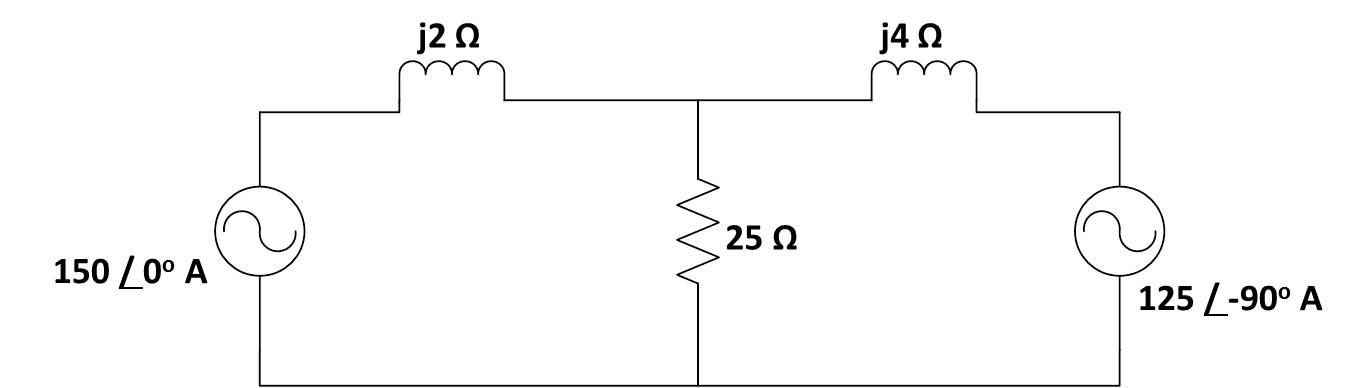
\includegraphics[width=0.7\textwidth]{Example1.jpg}
\caption{Circuit to accompany example 1}
\label{fig: Example1}
\end{figure}

\soln{6in}{
\begin{figure} [h!]
\centering
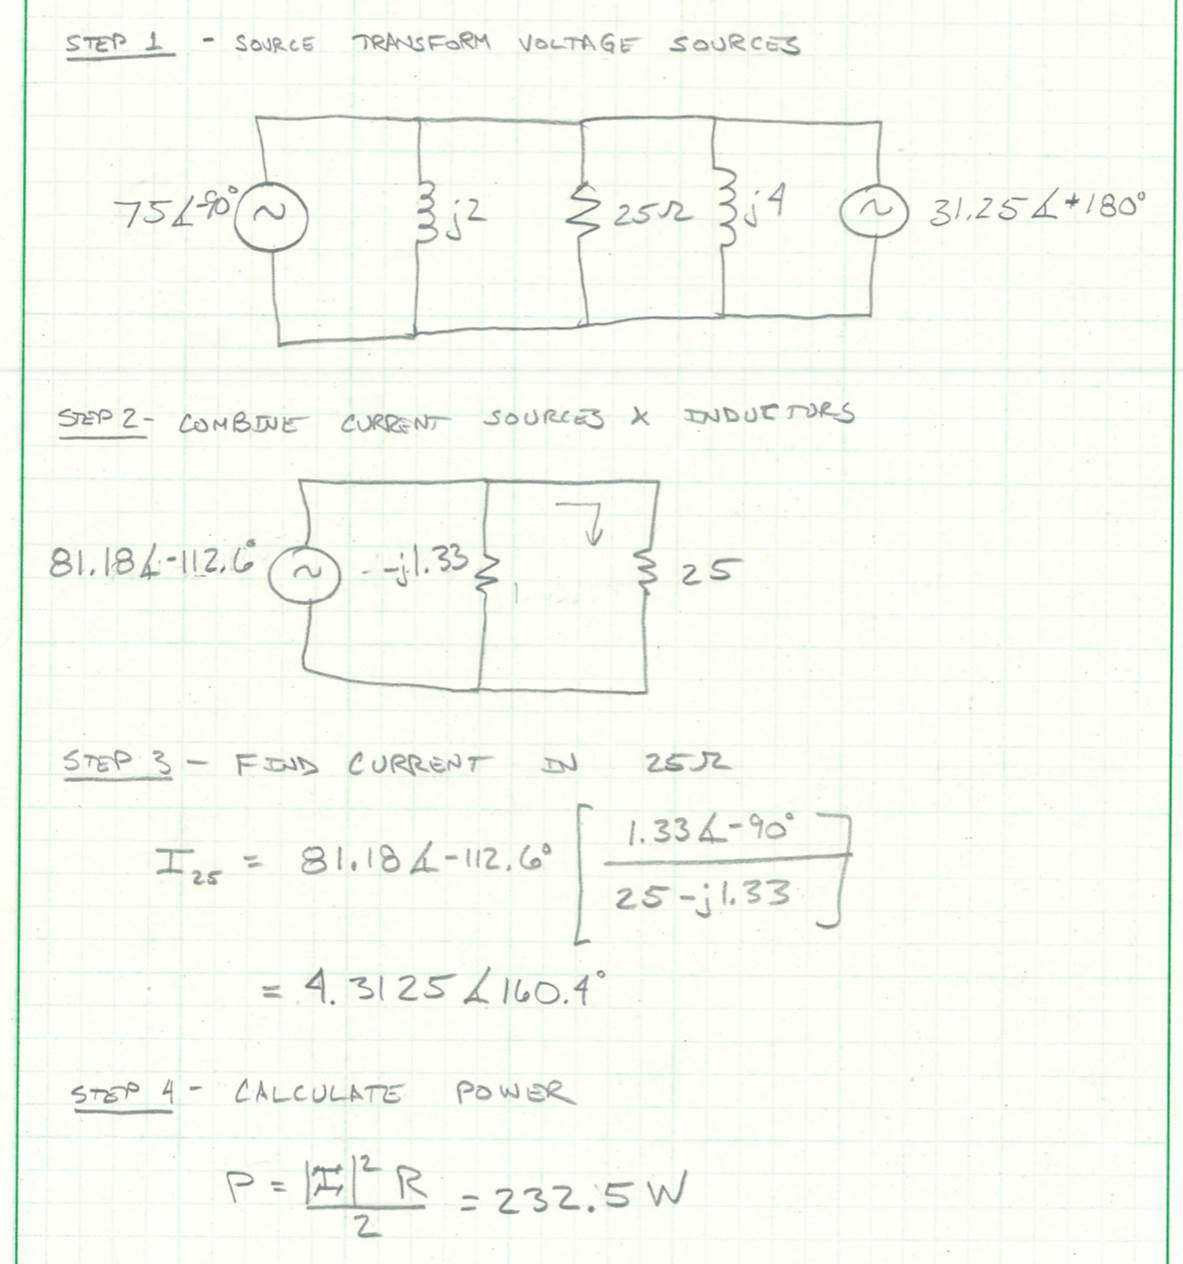
\includegraphics[width=0.9\textwidth]{Example1soln.jpg}
\end{figure}
}


\newpage
\clearpage
\pagebreak

\section{Maxumum Power Transfer}
Back in Lesson 10 we discussed the condition for maximum power transfer in purely resistive circuits.  Now we need to look at maximum power transfer for circuits with complex impedences.  We will start by looking at the Thevenin circuit shown in Figure \ref{fig: Thevenin}.  In this figure, $\mathbf{V_T}$ is a phasor source and the impedances are also complex.
\begin{figure} [h!]
\centering
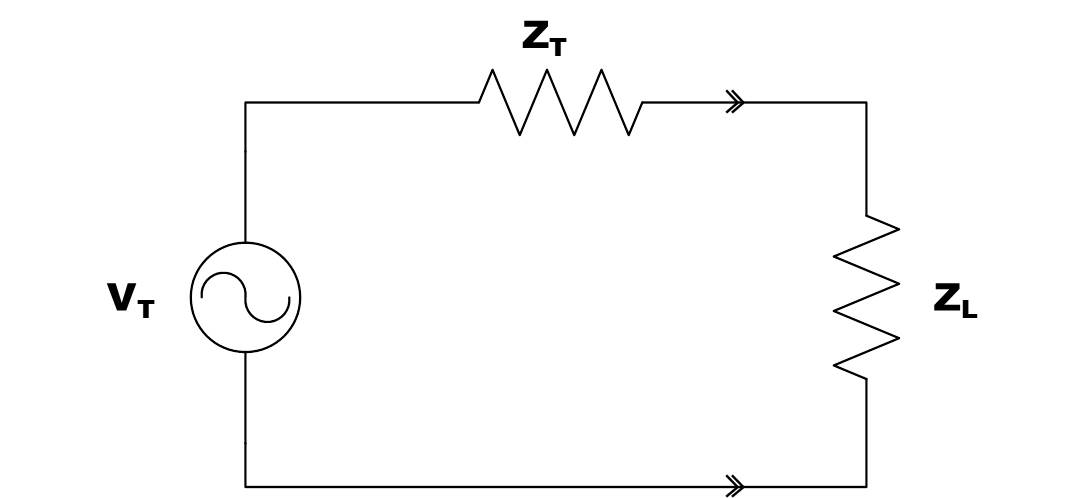
\includegraphics[width=0.5\textwidth]{Thevenin.jpg}
\caption{Thevenin circuit with complex source and impedances}
\label{fig: Thevenin}
\end{figure}

We will represent our complex impedances as
\soln{1in}{
\[
\mathbf{Z_T}=R_T+jX_T
\]
\[
\mathbf{Z_L}=R_L+jX_L
\]
}

We can write the current in this loop as:
\soln{2in}{
\[
\mathbf{I}=\frac{\mathbf{V_T}}{R_T+jX_T+R_L+jX_L}
\]
\[
\mathbf{I}=\frac{\mathbf{V_T}}{(R_T+R_L)+j(X_T+X_L)}
\]
}

For average power calculations we are really interested in the magnitude of the current which is
\soln{1in}{
\[
|\mathbf{I}| =\frac{|\mathbf{V_T}|}{\sqrt{(R_T+R_L)^2+(X_T+X_L)^2}}
\]
}

If we plug this result into our equation for average power, we get
\soln{2in}{
\[
P_{AVE} = \frac{R_L}{2}\frac{|\mathbf{V_T}|^2}{(R_T+R_L)^2+(X_T+X_L)^2}
\]
}

Using this equation, we want to select $R_L$ and $X_L$ to maximize $P_{AVE}$.  Remembering that reactances  are allowed to be negative, it should be obvious that choosing $X_L=-X_T$ will maximize $P_{AVE}$ for a given value of $R_L$.  This reduces our equation for average power to
\soln{2in}{
\[
P_{AVE} = \frac{R_L}{2}\frac{|\mathbf{V_T}|^2}{(R_T+R_L)^2}
\]
}

We will recall from Lesson 10, that power transfer is maximized when $R_L=R_T$; that is still true for complex impedances!

These to conditions combine to give us our condition for maximum power transfer to be:
\soln{1in}{
\[
R_T+jX_T=R_L-jX_L
\]
or
\[
Z_T=Z_L^*
\]
}

We can now use our average power formula from above to calculate maximum possible power transfer:
\soln{2in}{
\[
P_{AVE} = \frac{R_L}{2}\frac{|\mathbf{V_T}|^2}{(R_T+R_T)^2+(X_T-X_T)^2} = \frac{|\mathbf{V_T}|^2}{8R_T}
\]
}

\textbf{Example 2} -- Textbook Exercise 8-42 --- Calculate the maximum power available at the interface in Figure \ref{fig: Example2}.
\begin{figure} [h!]
\centering
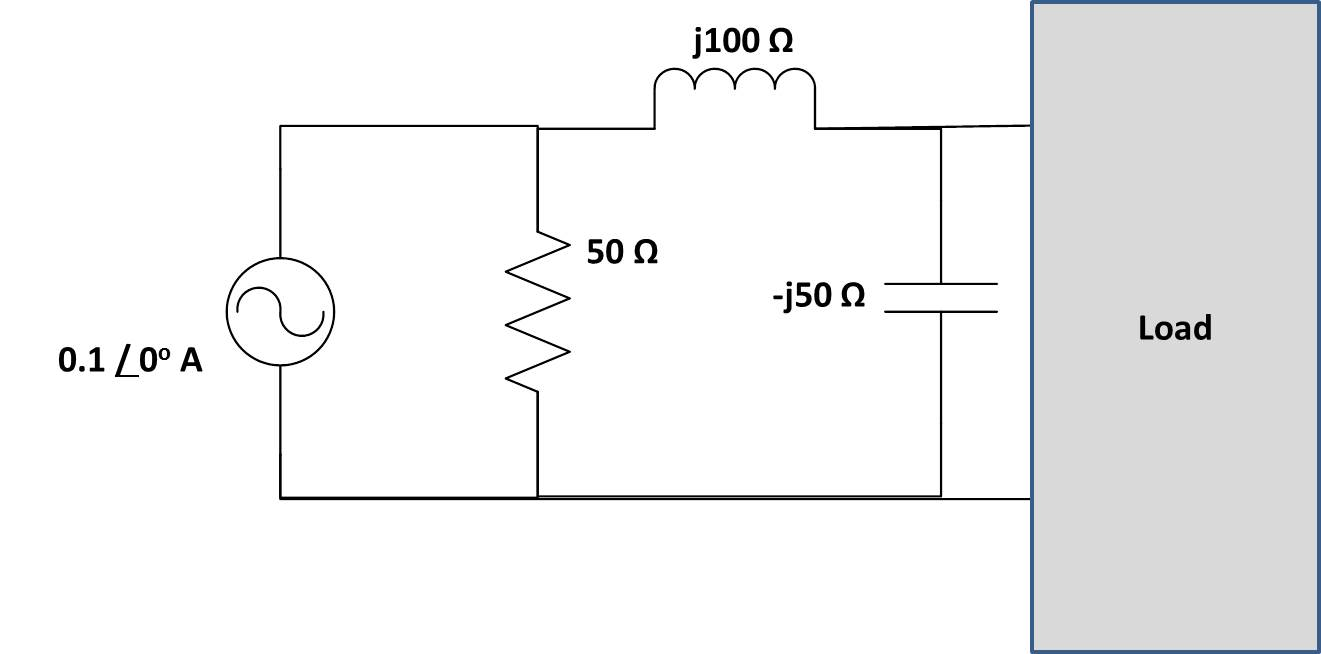
\includegraphics[width=0.6\textwidth]{Example2.jpg}
\caption{Circuit to accompany example 2}
\label{fig: Example2}
\end{figure}

\soln{6in}{
\begin{figure} [h!]
\centering
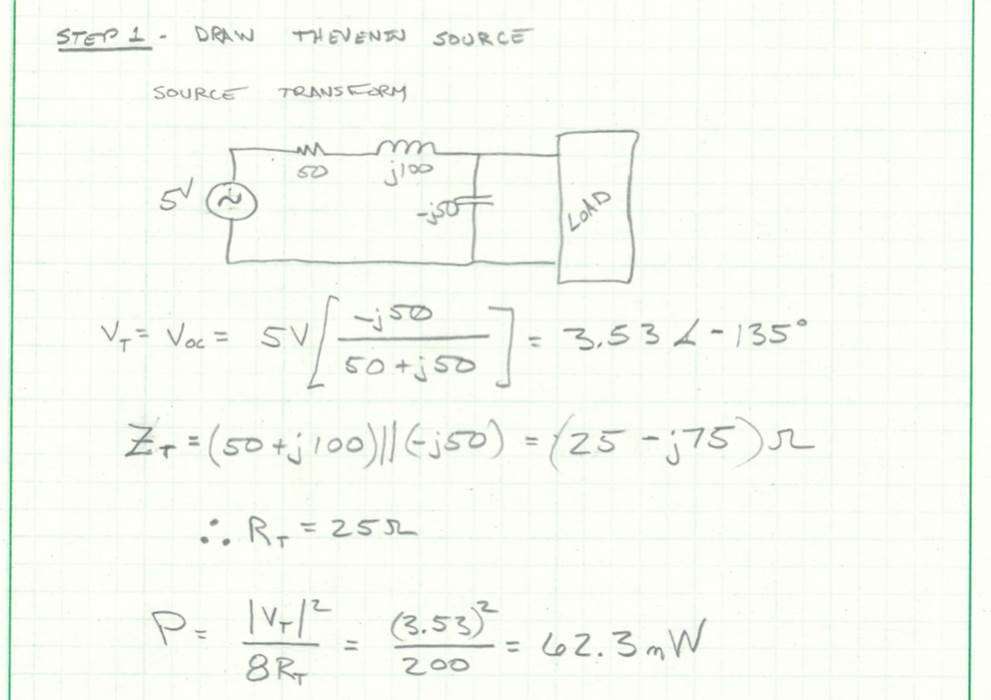
\includegraphics[width=0.8\textwidth]{Example2soln.jpg}
\end{figure}
}

\newpage
\clearpage
\pagebreak

\newpage
\clearpage
\pagebreak

\newpage
\clearpage
\pagebreak

\newpage
\clearpage
\pagebreak



\end{document}


% Equation Array Example Code
%\begin
%{eqnarray}
%P_R &=& i_R^2R \nonumber \\
%P_R &=& (100\ mA)^2 \times 100\ \Omega \nonumber \\
%P_R &=& (100 \times 10^{-3}\ A)^2 \times 100\ \Omega \\
%P_R &=& 10000 \times 10^{-6}\ A^2  \times 100\ \Omega \nonumber \\
%P_R &=& 1\ W  \nonumber
%\end{eqnarray}

% Figure Example Code
%\begin{figure} [h!]
%\centering
%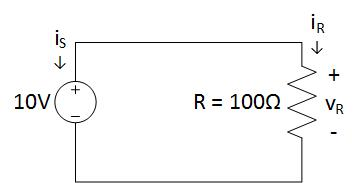
\includegraphics[width=0.5\textwidth]{OhmsLawExampleSolution.jpg}
%\caption{Ohm's Law example circuit}
%\label{fig: OhmsLawExampleSolution}
%\end{figure}

%Table Example Code
%\begin{table}[h]
%\centering
%\begin{tabular}{|l|c|c|}
%\hline
%Prefix & Abbreviation & Value \\
%\hline \hline
%Giga & $G$ & $10^9$ \\
%Mega & $M$ & $10^6$ \\
%Kilo & $k$ & $10^3$ \\
%\hline
%milli & $m$ & $10^{-3}$ \\
%micro & $\mu$ & $10^{-6}$ \\
%nano & $n$ & $10^{-9}$ \\
%pico & $p$ & $10^{-12}$ \\
%\hline
%\end{tabular}
%\caption{Engineering prefixes and values}
%\label{tab: Eng Prefixes}
%\end{table}
